\chapter{Introduction}

% Foreword
%
% context (focus on anyone) why now? - current situation, and why the need is so important
Since parallel computing is again becoming a topic of interest in computer science, it is important to revisit the theoretical foundations of highly parallel computing.
% need (focus on readers) why you? - why this is relevant to the reader, and why something needed to be done
``Inherently sequential'' computational problems see no significant speedup when run on highly parallel computers.
Just as there are efficient approximations for intractable optimization problems, so too are there efficient and highly parallel approximations for optimization problems that are tractable but inherently sequential.
%% (From here forward, we write ``parallel'' instead of ``efficient and highly parallel'' and ``sequential'' instead of ``inherently sequential''\kern-0.5em.\kern0.25em)
%%% relevant existing work, given as part of the need
For example, the problem of computing the optimal vector in a positive linear program, a problem relevant to distributed flow control within a network of routers, is inherently sequential, but a vector very close to the optimal one can be computed quickly in parallel.
Similarly, just as there are fixed-parameter tractable algorithms for some intractable problems, so too are there fixed-parameter parallel algorithms for some sequential parameterized problems.
For example, \todo{this section was only reviewed up to this point. Updates needed below. }
% task (focus on author) why me? - what was undertaken to address the need
We develop the theory of structural complexity for highly parallel algorithms for tractable but inherently sequential problems in decision problems, optimization problems, and parameterized problems.
This area has not been well-studied, and when it has been studied, the results focus mostly on parallel algorithms for \emph{intractable} problems, (that is, $\NC$ algorithms for $\NP$-complete problems), not parallel algorithms for tractable sequential problems (that is, $\NC$ algorithms for $\P$-complete problems).
% object (focus on document) why this document - what the document covers
This prospectus describes work we have already completed and work that remains in developing this theory.

% Summary
%
% findings (focus on author) what? - what the work revealed when performing the task
The two sections below discuss two main approaches to proving the limitations of parallel approximations for sequential problems.
The first section discusses the complexity classes associated with parallel approximation algorithms, the second discusses augmenting a parallel algorithm with a small amount of nondeterminism as a technique to prove approximability or inapproximability of sequential problems.
Both concern inapproximability by $\NC$ algorithms, but the former considers $\P$ optimization problems while the latter considers $\NNC(\polylog)$ problems.
% conclusion (focus on readers) so what? - what the findings mean for the audience
Together, these form the basis for proving approximability and inapproximability for tractable sequential problems by parallel algorithms.
% perspective (focus on anyone) what now? - what should be done next
This line of research, along with the fact that the complexity of solving a computational problem exactly seems to have little to with the approximability of that problem, emphasizes the need to further determine the relative difficulty of computational problems with respect to the complexity of decision, verification, and approximation.

\section{more infoooooo}

We study the structural complexity of sequential versus parallel computation in decision problems, optimization problems, and parameterized problems.
Decision problems lead to the other two kinds of problems by modifying either the solution space or the resource usage bounds.
Optimization problems generalize decision problems by allowing a search for a good solution among many candidates.
Parameterized problems generalize decision problems by allowing resource bounds to depend on a parameter of the problem instance instead of simply the size.
The study of the computational complexity of both optimization problems and parameterized problems provide more details about the complexity than does the study of only the decision complexity.

\begin{minipage}[t]{0.31\linewidth}
  \centering
  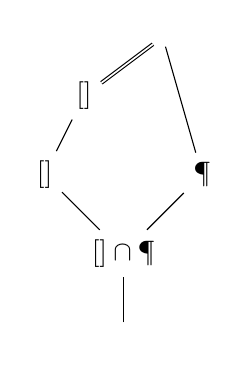
\begin{tikzpicture}
  \node at (0, 0) (nc) {$\NC$};
  \node at (0, 1) (both) {$\NNC[\polylog] \cap \P$};
  \node at (-1, 2) (nncpolylog) {$\NNC[\polylog]$};
  \node at (1, 2) (p) {$\P$};
  \node at (0.5, 3.75) (np) {$\NP$};
  \node at (-0.5, 3) (nnc) {$\NNC[\poly]$};

  \draw (nc) to (both);
  \draw (both) to (nncpolylog);
  \draw (both) to (p);
  \draw (p) to (np);
  \draw (nncpolylog) to (nnc);
  \draw[double] (nnc) to (np);
\end{tikzpicture}

\end{minipage}%
\begin{minipage}[t]{0.31\linewidth}
  \centering
  \begin{tikzpicture}
  \node at (0, 0) (nco) {$\NCO$};
  \node at (0, 1) (both) {$\ApxNCO \cap \PO$};
  \node at (-1, 2) (apxnco) {$\ApxNCO$};
  \node at (1, 2) (po) {$\PO$};
  \node at (0.5, 3.75) (npo) {$\NPO$};
  \node at (-0.5, 3) (nnco) {$\NNCO$};

  \draw (nco) to (both);
  \draw (both) to (apxnco);
  \draw (both) to (po);
  \draw (po) to (npo);
  \draw (apxnco) to (nnco);
  \draw[double] (nnco) -- (npo) node [rotate=45, midway] {\small$/$};
\end{tikzpicture}

\end{minipage}%
\begin{minipage}[t]{0.31\linewidth}
  \centering
  \begin{tikzpicture}
  \node at (0, 0) (fpnc) {$\para \NC$};
  \node at (0, 1) (both) {$\para \WNC[1] \cap \para \P$};
  \node at (-1, 2) (dontknow) {$\para \WNC[1]$};
  \node at (1, 2) (fpt) {$\para \P$};
  \node at (0.5, 3.75) (wp) {$\para \WP$};
  \node at (-0.5, 3) (wpp) {$\para \WNC$};

  \draw (fpnc) to (both);
  \draw (both) to (dontknow);
  \draw (both) to (fpt);
  \draw (fpt) to (wp);
  \draw (dontknow) to (wpp);
  \draw (wpp) to (wp);
\end{tikzpicture}

\end{minipage}

These inclusion diagrams shape how we approach all the problems in this paper.
Double lines represent equality, solid lines represent strict inequality under some reasonable complexity-theoretic assumptions, and dashed lines represent inclusions of unknown strictness or equality.
The fact that $\NNC[\poly] = \NP$ but $\NNCO \neq \NPO$ and $\para \WNC \neq \para \WP$ (under the assumption $\NC \neq \P$) leads us to conclude that viewing a computational problem as merely a decision problem is too coarse-grained an approach---it does not give enough information about the computational complexity of the problem.

There is another view that we approach only indirectly in this work, the complexity of verification.
This is why $\NNCO$ differs from $\NPO$ and $\para \WNC$ differs from $\para \WP$: these classes take into account the complexity of verifying a solution.
The classes of decision problems $\NNC[\poly]$ and $\NP$ do not.

\todo{Descriptive complexity encompasses all of these; specifically for parallel complexity of optimization problems, see \autocite{kt93}.}

We aim to show that there is a $\P$-complete problem that is also
\begin{enumerate}
\item[(D1)] not in $\NNC[\polylog]$ (\autocite[Theorem~3.9]{ncpcp} provides one unless $P \subsetneq \polyL$),
\item[(D2)] in $\NNC[\polylog]$ but not in $\NC$ (unknown),
\item[(O1)] not in $\ApxNCO$ (\autocite[Theorem~3.25]{ncapproximation} provides one unless $\NC = \P$),
\item[(O2)] in $\ApxNCO$ but not in $\NCO$ (\autocite[Theorem~3.25]{ncapproximation} provides on unless $\NC = \P$),
\item[(P1)] not in $\para \WNC[1]$ (unknown),
\item[(P2)] in $\para \WNC[1]$ but not in $\para \NC$ (unknown).
\end{enumerate}

\section{Outline}

The referenced theorems correspond to the theorems in the respective papers.

\paragraph{Decision Problems.}
Completed:
\begin{enumerate}
\item $\NC = \PCP[O(\log \log n, O(1)]$ (Theorem~3.3).
\item $\NNC[\polylog] = \PCP[O(\log \log n), \polylog]$ (Corollary~3.2).
\item $\NP = \PCP[O(\log n), O(1)]$ (Theorem~3.4).
\item negative consequences $\PCP$ hierarchy collapses (Corollary~3.6) (\emph{relates to parameterized problems})
\item consequences of $\P = \PCP[O(\log \log n), \polylog]$ (Theorem~3.9).
\end{enumerate}
To-do:
\begin{enumerate}
\item \textbf{Low priority:} Inapproximability of the High Degree Subgraph problem (Section~4) (\emph{relates to optimization problems}).
\end{enumerate}

\paragraph{Optimization problems.}

Completed:
\begin{enumerate}
\item $\NNCO$-complete problem (Theorem~3.3).
\item $\NPO$-complete problem (Corollary~3.4).
\item $\NNCO = \NPO \iff \NC = \P$ (Theorem~3.5).

\item $\PO$-complete problem (Theorems~3.8 and 3.9).
\item $(\PO \cap \NNCO)$-complete problem (Corollary~3.11).
\item $\PO \cap \NNCO = \PO \iff \NC = \P$ (Theorem~3.12).

\item $\PO \cap \NNCO$ is not closed under $\leq_m^{AP}$ reductions (Corollary~3.10).

\item Strictness of $\NNCO$ approximation hierarchy (Theorem~3.24).
\item Strictness of $\PO \cap \NNCO$ approximation hierarchy (Theorem 3.25).
\end{enumerate}
To-do:
\begin{enumerate}
\item \textbf{Low priority:} $\ApxNCO$-complete problem (Section~3.3).
\item \textbf{High priority:} descriptive complexity characterization of $\ApxNCO$ (Section~4) (\emph{relates to parameterized problems}).
\item \textbf{High priority:} reduction preserving both verification complexity and approximability.
\end{enumerate}

\paragraph{Parameterized problems.}
Completed:
\begin{enumerate}
\item Circuit value problem is $\P$-complete but in $\para \AC^{0 \uparrow}$ (Theorems~3.3 and 3.5).
\item Nonuniform circuits for proving $\NC = \NNC[i(n) \log n] \implies \para \NC = \para \WNC$.
\item $\mathcal{O} \in \ENCAS \implies p \dash \mathcal{O} \in \para \NC$ (Theorem~3.18)
\item $\para \P$-complete problems (Section~4.2).
\item Definition of $\para \WNC[t]$?
\item $\para\NC = \para \WNC[t] \iff \Pi_t\LOGTIME[i(n) \log n] \subseteq \NC^d$, if it's correct (Section~6.4).
\end{enumerate}
To-do:
\begin{enumerate}
\item \textbf{High priority:} extend \autocite[Corollary~3.8]{est15} to $\para \WNC^d \subseteq \para \P$ implies $\W[\NC^d \textsc{sat}] = \para \P$?
\item \textbf{Very high priority:} show that collapses in the inclusion chain $\para \WNC^1$ through $\para \WP$ imply corresponding collapses in decision problems? This should follow from ``Describing parameterized complexity classes'' by Flum and Grohe (Section~5.6) (\emph{relates to decision problems}).
\item \textbf{Low priority:} provide descriptive complexity characterizations of the $\para \W \mathcal{C}$ classes?
\item \textbf{High priority:} $\para \WNC^1[t] \subseteq \para \P$ if and only if a class between $\W[t] = \para \P$?
\end{enumerate}
